
\chapter{Cadenas de texto}
\label{strings}
\index{string}

Las cadenas de texto no son como los enteros, los racionales,
y los Booleanos. Una cadena de texto es una {\bf secuencia} de caracteres,
lo cual significa que es una colección ordenada de otros valores,
y algunas veces necesitas acceder algunos de estos valores individuales.
En este capítulo verás cómo analizar, manejar, y modificar cadenas
de texto, y aprenderás sobre algunos de los métodos que las
cadenas de texto proveen. También aprenderás sobre una
herramienta muy poderosa para la manipulación de texto, 
expresiones regulares (también conocidas como ``regexes``).
\index{sequence}
\index{regex}


\section{Una Cadena de Texto es una Secuencia}

\index{sequence}
\index{character}
\index{bracket operator}
\index{operator!bracket}
Una cadena de texto es primariamente una pieza de datos textuales,
pero es técnicamente una secuencia ordenada de caracteres.

Muchos lenguajes de programación te permiten acceder caracteres
individuales de una cadena de texto con índice entre corchetes. 
Esto no es directamente posible en Perl, pero todavía puedes
los caracteres uno a la vez usando el método integrado {\tt comb} 
y el operador corchete:

\begin{verbatim}
> my $cadena = "banana";
banana
> my $cad = $cadena.comb;
(b a n a n a)
> say $cad[1];
a
> say $cad[2];
n
\end{verbatim}
%
El método {\tt comb} en la segunda sentencia divide la cadena de texto
en una lista de caracteres que puedes acceder individualmente con
los corchetes.
\index{comb function and method}
\index{method!comb}
\index{function!comb}
\index{bracket!square}
\index{square bracket operator}
\index{index}
\index{subscript}

La expresión dentro de los corchetes se llama un {\bf índice}
(también llamado subíndice). El índice indica cuales 
caracteres en la secuencia quieres (de ahí el nombre). Pero
puede ser que esto no es lo que esperabas: el artículo con
índice 1 es la segunda letra de la palabra. Para los
científicos de la computación, el índice es usualmente
un desplazo del inicio. Por ejemplo, el índice de la primera 
letra (``b``) es 0, y el índice de la primera ``a`` es 1,
no 2, etcétera.
\index{index!starting at zero}
\index{zero, index starting at}

También podrías extraer una ``rebanada`` de varios caracteres
de una sola vez al usar el operador de rango dentro de los 
corchetes:
\index{slice}

\begin{verbatim}
> say $cad[2..5]
(n a n a)
\end{verbatim}
%
\index{substring}
De nuevo, la subcadena ``nana`` comienza en la tercera letra
de \verb|'banana'|, pero esta letra está indexada 2, y la
sexta letra tiene índice 5.

Aunque esto puede ser útil en ocasiones, esta no es la manera
en la que manejarías cadenas de texto en Perl, el cual tiene
herramientas superiores que son más poderosas y más 
expresivas, así que raramente necesitas usar índices o 
subíndices para acceder caracteres individuales.

También, si existe una necesidad real de acceder y manipular
las letras individuales, haría más sentido almacenarlas en un 
array, pero no hemos hablado sobre arrays todavía, así que
regresaremos a esto más tarde.

\section{Operadores Comunes de Cadenas de Texto}
\index{string!operators}

Perl provee un número de operadores y funciones para el 
manejo de cadenas de texto. Revisemos algunos de los más 
populares.

\subsection{Longitud de una Cadena de Texto}
\index{chars function}
\index{function!chars}
\index{string!length}

La primera cosa que desearíamos saber sobre una cadena de texto 
es su longitud. El método (o función) {\tt chars} devuelve el número de
caracteres de una cadena de texto. Como podemos ver, {\tt chars} puede
usarse con una sintaxis de método o función:
\index{invocation!method}
\index{method invocation}

\begin{verbatim}
> say "banana".chars;   # sintaxis de invocación de método
6
> say chars "banana";   # sintaxis de llamada de función
6
\end{verbatim}
%

\index{Unicode}
\index{grapheme}
Nota que, con el advenimiento de Unicode, la noción 
sobre la longitud de una cadena de texto se ha vuelto 
más complicada que lo era con cadenas de texto ASCII.
Hoy en día, un carácter puede estar compuesto de uno, dos, o 
más bytes. La rutina {\tt chars} devuelve el número de 
caracteres (en el sentido de los grafemas de Unicode, los cuales
son más o menos lo que los humanos perciben como caracteres) dentro
de la cadena, aún cuando algunos caracteres requieren una
codificación de más de 2, 3, o 4 bytes.

Una cadena de texto con una longitud cero (i.e., sin caracteres) se
conoce como una \emph{cadena de texto vacía}.

\subsection{Búsqueda de una Subcadena Dentro de una Cadena de Texto}
\label{find}
\index{index function}
\index{function!index}
\index{substring}

La función integrada {\tt index} usualmente toma dos argumentos,
una cadena de texto y una subcadena (algunas veces conocidas como
la ``paja`` y la ``aguja``), busca la subcadena en la cadena de texto,
y devuelve la posición donde se encuentra la subcadena. Si la subcadena
no se encuentra en la cadena, la función devuelve un valor indefinido:

\begin{verbatim}
> say index "naranja", "ra";
2
> say index "naranja", "je";
Nil
\end{verbatim}
%

\index{offset}
Nuevamente, el índice es un desplazo del inicio de la cadena 
de texto, así que el índice de la primera letra (``n``) es cero,
y el índice de la segunda ``a`` es 3, no 4.
\index{index!starting at zero}

También puedes invocar a {\tt index} con una sintaxis de método:
\begin{verbatim}
> say "naranja".index("ra");
2
\end{verbatim}
%

La función {\tt index} puede tomar un tercer argumento opcional,
un entero que indica donde comenzar la \emph{búsqueda} (y por lo
tanto ignorando en la búsqueda cualquier carácter posterior a
la posición de inicio):

\begin{verbatim}
> say index "naranja", "a", 2;
3
\end{verbatim}
%
Aquí la función {\tt index} comenzó la búsqueda en la ``r`` y encontró 
la posición de la segunda ocurrencia de la subcadena ``a``.
 

\index{function!rindex}
\index{rindex function}
También existe una función {\tt rindex}, la cual realiza la búsqueda
de la subcadena de atrás hacia adelante y devuelve la última posición de 
la subcadena dentro de la cadena de texto:

\begin{verbatim}
> say rindex "naranja", "a";
6
\end{verbatim}
%

Nota que aunque {\tt rindex} inspecciona la cadena de texto
de atrás hacia adelante, la función devuelve una posición
computada desde el inicio de la cadena de texto.

\subsection{Extrayendo una Subcadena de una Cadena de Texto}
\index{substr function or method}
\index{function!substr}
\index{substring}

La función opuesta a {\tt index} es la función (o método) {\tt substr},
la cual, dada una posición inicial y una longitud, extrae una subcadena
de una cadena de texto:

\begin{verbatim}
> say substr "Hacer es la mejor manera de decir.", 0, 5;
Hacer
> say "Hacer es la mejor manera de decir.".substr(12, 5)
mejor
\end{verbatim}
%

\index{chars function}
\index{Unicode}
\index{grapheme}
Nota que, al igual que la función {\tt chars}, la longitud es
expresada en caracteres (o grafemas Unicode), no en bytes.
De igual modo, como puedes observar, los espacios que separan
las palabras dentro de la cadena de texto obviamente cuentan 
como caracteres. El argumento de la longitud es opcional; 
si no se provee, la función {\tt substr} devuelve la subcadena
comenzando en la posición de inicio al final de la cadena de texto:

\begin{verbatim}
> say "Hacer es la mejor manera de decir.".substr(9)
la mejor manera de decir.
\end{verbatim}

Similamente, si el valor de la longitud es muy largo para que 
la subcadena comience en la posición inicial, la función
{\tt substr} devolverá la subcadena comenzando en la posición
inicial hasta el final de la cadena:

\begin{verbatim}
> say substr "banana", 2, 10;
nana
\end{verbatim}

Por supuesto, los parámetros de la posición inicial y la longitud 
no necesitan números literales como en los ejemplos anteriores; puedes
también usar variables (o hasta una expresión o una función que devuelve 
un valor numérico), provisto que la variable o la función pueda ser 
coaccionada en un entero. Pero la posición de inicio debe estar dentro 
del rango de la cadena de texto, y si falla obtienes un error 
{\tt Start argument to substr out of range ...}; por lo tanto
podrías tener que verificarlo en contra de la longitud de la 
cadena de texto con antelación.

También puedes comenzar a contar de atrás hacia adelante con la
siguiente sintaxis:

\begin{verbatim}
> say "I have a dream".substr(*-5)
dream
> say substr "I have a dream", *-5;
dream
\end{verbatim}
%
Aquí, el asterisco * puede considerarse como una representación de la
longitud total de la cadena de texto; \verb|*-5| es por lo tanto la posición
en la cadena de texto cinco caracteres antes del final de la cadena. Así que
\verb|substr(*-5)| devuelve los caracteres desde esa posición hasta el final
de la cadena de texto, i.e., los últimos cinco caracteres de la cadena de
texto.
\index{substr function}
\index{substring}

\subsection{Otras Funciones o Métodos Útiles de Cadenas de Texto}
\index{string!operators}

Esto puede no ser obvio todavía, pero prontamente veremos
que la combinación de las funciones de cadenas de texto que discutimos
más arriba nos dan ya mucho poder para manipular cadenas de texto
más allá de lo que piensas posible en este punto.

Déjanos mencionar brevemente varias funciones adicionales
que pueden ser útiles de vez en cuando.

\subsubsection{flip}

\index{flip function}
\index{function!flip}
La función (o método) {\tt flip} invierte una cadena de texto:

\begin{verbatim}
> say flip "mango";
ognam
\end{verbatim}
%

\subsubsection{split}
\index{split function or method}
\index{function!split}
\index{delimiter}
La función (o método) {\tt split} divide una cadena de texto 
en subcadenas de texto, basado en los delimitadores en l
cadena de texto:

\begin{verbatim}
> say $_ for split "-", "25-12-2016";
> #                 ^ delimitador
25
12
2016
> for "25-12-2016".split("-") -> $val {say $val};
25
12
2016
\end{verbatim}

El delimitador puede ser un solo carácter con comillas como
en el ejemplo más arriba o una cadena de varios caracteres, 
tales como una coma y un espacio en el ejemplo más abajo:

\begin{verbatim}
> .say for split  ", ", "Jan, Feb, Mar";
> #                ^^ delimitador
Jan
Feb
Mar
\end{verbatim}

Recuerda que \verb|.say| es un atajo para \verb|$_.say|.

Por defecto, los delimitadores no aparecen en la salida producida por 
la función (o método) {\tt split}, pero este comportamiento puede 
cambiarse con el uso de {\tt adverbio} apropiado. Un adverbio es básicamente
un argumento nombrado de una función que modifica la manera en la 
función se comporta. Por ejemplo, el adverbio {\tt :v} (valores)
le dice a {\tt split} que también devuelva el valor del delimitador:
\index{adverb}
\index{:v adverb}

\begin{verbatim}
> .perl.say for split  ', ', "Jan, Feb, Mar", :v;
"Jan"
", "
"Feb"
", "
"Mar"
\end{verbatim}

Los otros adverbios que pueden usarse en este contexto son {\tt :k} (claves), 
{\tt :kv} (claves y valores), y {\tt :p} (pares). Su significados detallados pueden
encontrarse en la documentación para {\tt split}
(\url{https://docs.perl6.org/routine/split}). El adverbio {\tt skip-empty}
remueve las partes vacías de la lista de resultados.

La función {\tt split} pueden también usarse un \emph{patrón} 
de expresión regular como un delimitador, y esto puede hacerla
mucho más poderosa. Estudiaremos expresiones regulares más adelante
en este capítulo.
\index{regular expression}
\index{regex}

\subsubsection{Concatenación de Cadenas de Texto}

\index{concatenate operator}
\index{string!concatenation}
\index{string concatenation}

El operador \verb|~| concatena dos cadenas de texto y forma una:

\begin{verbatim}
> say "ban" ~ "ana";
banana
\end{verbatim}
%

Puedes tener cadenas de varias ocurrencias de este operador
para concatenar más de dos cadenas:

\begin{verbatim}
> say "ba" ~ "na" ~ "na";
banana
\end{verbatim}
%

Si se usa como un operador prefijo unario,
\verb|~| transforma su argumento en una cadena de texto:
\index{stringify operator}
\index{stringification}

\begin{verbatim}
> say (~42).WHAT;
(Str)
\end{verbatim}
%

\subsubsection{Separando en Palabras}

\index{words function or method}
La función {\tt words} devuelve una lista de palabras
que componen la cadena de texto:

\begin{verbatim}
> say "I have a dream".words.perl;
("I", "have", "a", "dream").Seq
> .say for "I have a dream".words;
I
have
a
dream
\end{verbatim}
%

\subsubsection{join}

\index{join function or method}
\index{function!join}
La función {\tt join} toma un argumento separador y una lista
de cadenas de texto como argumentos; la función las intercala
con el separador, concatena todo en una sola cadena de texto, y 
devuelve la cadena de texto resultante.

Este ejemplo ilustra el uso de las funciones (o métodos) 
{\tt words} y {\tt join}:

\begin{verbatim}
say 'I have a dream'.words.join('|');    # -> I|have|a|dream
say join ";", words "I have a dream";    # -> I;have;a;dream
\end{verbatim}
%

\index{words function or method}
En ambos casos, {\tt words} primero divide la cadena original
en una lista de palabras,  {\tt splits} sutura los artículos
de esta lista y los devuelve en una nueva cadena de texto 
intercalados con el separador.

\subsubsection{Conversión a Minúscula y a Mayúscula}
\index{lc function or method} 
\index{lower case!lc function}
\index{uc function or method}
\index{tc function or method}
\index{upper case}
\index{lower case}
\index{title case}
\index{case!upper}
\index{case!lower}
\index{case!title}

Las rutinas {\tt lc} y {\tt uc} devuelven respectivamente
una versión en minúscula y una versión mayúscula de sus 
argumentos. También está la función {\tt tc} la cual devuelve
su argumento con la primera letra en mayúscula:

\begin{verbatim}
say lc "Abril";    # -> april
say "Abril".lc;    # -> april
say uc "abril";    # -> APRIL
say tc "abril";    # -> April
\end{verbatim}

\index{eq, string equality operator}
Recuerda que el operador {\tt eq} chequea la igualdad de dos 
cadenas de texto.

\section{Recorrido de una Cadena con un bucle {\tt while} o {\tt for}}
\label{stringtraversal}
\index{traversal}
\index{loop!traversal}
\index{for loop}
\index{loop!for}
\index{statement!for}
\index{index function}
\index{while loop}

Muchas computaciones involucran el procesamiento de una
cadena de texto una carácter a la vez. Usualmente ellas
comienzan al principio, seleccionan cada carácter en turno,
hacen algo con dicho carácter, y continúan hasta el final.
Este patrón de procesamiento se conoce como {\bf recorrido}. 
Una manera de escribir un recorrido es con un bucle {\tt while}
y la función {\tt index}:
\index{while loop}
\index{index}

\begin{verbatim}
my $indice = 0;
my $fruta = "banana";
while $indice < $fruta.chars { 
    my $letra = substr $fruta, $indice, 1; 
    say $letra; 
    $indice++;
}
\end{verbatim}
%

Esto imprimirá cada letra, una a la vez:
\begin{verbatim}
b
a
n
a
n
a
\end{verbatim}
%
Este bucle recorre la cadena de texto y muestra cada letra
en un línea por si misma. La condición del bucle es 
{\tt \$indice < \$fruta.chars},
así que cuando {\tt \$indice} es igual a la longitud de
la cadena de texto, la condición es falsa, y el cuerpo del
bucle no se ejecuta. En otras palabras, el bucle para cuando
{\tt \$indice} es la longitud de la cadena de texto menos 
uno, lo cual corresponde al último carácter de la cadena 
de texto.

Como ejercicio, escribe una función que toma una cadena de 
texto como un argumento y muestra las letras de atrás hacia
adelante, una por línea. Hazlo por lo menos una vez sin utilizar
la función {\tt flip}. Solución: \ref{sol_stringtraversal}

Otra forma de escribir un recorrido es con un bucle {\tt for}:
\index{for loop}
\index{comb function and method}

\begin{verbatim}
my $fruta = "banana";
for $fruta.comb -> $letra {
    say $letra
}
\end{verbatim}
%

Cada vez a través del bucle, el siguiente carácter en la
cadena de texto es asignado a la variable {\tt \$letra}.
El bucle continúa hasta que no hayan más caracteres.

El bucle podría también usar la función {\tt substr}:
\index{index function}

\begin{verbatim}
for 0..$fruta.chars - 1 -> $indice {
    say substr $fruta, $indice, 1;
}
\end{verbatim}
%

\index{concatenation}
\index{abecedarian}
\index{aphabetic order}
\index{McCloskey, Robert}

El siguiente ejemplo muestra cómo usar concatenación y
un bucle {\tt for} para genera una serie de abecedario (
es decir, en orden alfabético). En el libro 
{\em Make Way for Ducklings} de McCloskey, los nombres de los
patitos son Jack, Kack, Lack, Mack, Nack, Ouack, Pack, y Quack. 
Este bucle podría muestra estos nombres en orden:

\begin{verbatim}
my $sufijo = 'ack';
for 'J'..'Q' -> $letra {
    say $letra ~ $sufijo;
}
\end{verbatim}
%
La salida es:

\begin{verbatim}
Jack
Kack
Lack
Mack
Nack
Oack
Pack
Qack
\end{verbatim}
%
Por supuesto, esto no es del todo correcto dado que ``Ouack'' y 
``Quack'' están mal escritos. Como ejercicio, modifica el programa
para arreglar este error. Solución: \ref{sol_ducklings}.


\section{Bucles y Conteo}
\label{counter}
\index{counter}
\index{counting and looping}
\index{looping and counting}
\index{looping!with strings}

El siguiente programa cuenta el número de veces que 
la letra ``a`` aparece en una cadena de texto:
\index{comb function and method}

\begin{verbatim}
my $palabra = 'banana';
my $conteo = 0;
for $palabra.comb -> $letra {
    $conteo++ if $letra eq 'a';
}
say $conteo;              # -> 3
\end{verbatim}
%

\index{counter}
Este programa demuestra otro patrón de la computación 
llamado {\bf contador}. La variable \verb|$conteo| se inicializa
a 0 y después se incrementa por uno cada vez que se encuentra
una ``a``. Cuando el bucle termina, \verb|$conteo| contiene
el resultado---el número total de ocurrencias de la letra ``a``.
\index{incrementation}

\index{encapsulation}
Como ejercicio, encapsula este código en una subrutina llamada
{\tt contar}, y generalízala para que acepte una cadena de texto 
y la letra a contar como argumentos. Solución: \ref{sol_count_letters}.
\label{count_letters}

\section{Expresiones Regulares (Regexes)}
\label{regex}
\index{regex}
\index{regular expression}

Las funciones y los métodos de cadenas de texto que hemos visto
hasta ahora son realmente poderosos, y pueden usarse para un 
sin número de operaciones relacionadas con la 
manipulación de cadenas de texto. Pero supón que quieres extraer
de la cadena ``yellow submarine`` cualquier letra después
de la letra ``l`` y antes de la letra ``w``. Este tipo de 
``búsqueda difusa`` puede hacerse con un bucle, pero no 
es práctico. Puedes hacerlo como un ejercicio si deseas,
pero debo advertirte: es algo delicado y difícil. Aún si 
no lo haces, la solución puede interesarte: 
ver Subsección\ref{sol_regex_loop}. 
\label{regex_loop}

Si agregas otra condición, por ejemplo que esta letra 
debería extraerse o \emph{capturarse} (i.e. almacenada para 
uso futuro) solo si el resto de la cadena de texto contiene
la subcadena ``rin``, esto comienza a ser algo tedioso. También,
cualquier cambio a los requerimientos conduce a que tengamos
que hacer una reescritura substancial o hasta refactorizar
el código completamente.

Para este tipo de trabajo, una {\bf expresión regular} 
o un {\bf regex} es una herramienta mucha más poderosa
y expresiva. La siguiente es una manera de extraer letras usando
el criterio descrito anteriormente: 


\begin{verbatim}
> my $cadena = "yellow submarine";
yellow submarine
> say ~$0 if $cadena ~~ / l (.) w .*? rin /;
o
\end{verbatim}

No te preocupes si no entiendes este ejemplo;
afortunadamente todo se aclarará muy pronto.

\index{operator!smart match}
\index{smart match operator}
El operador \verb|~~| se conoce como el operador de coincidencia
inteligente. Es un operador de relación muy poderoso que puede
usarse para tareas de comparación más avanzadas. En este caso, 
el operador chequea si la variable {\tt \$cadena} a su izquierda
``coincide`` con la expresión a su derecha, i.e., como una 
primera aproximación, si la expresión a su derecha describe la 
cadena de texto (o parte de la misma).

\index{pattern}
La parte \verb|/ l (.) w .*? rin /| se llama un patrón de regex y puede
describirse así: la letra ``l``, seguida por cualquier otro carácter (el
punto) para ser capturado (gracias a los paréntesis), seguida por la
letra ``w``, seguida por un número no específico de caracteres,
seguida por la subcadena ``rin``. ¡Uff! ¡Todo esto en una sola línea
de código! Bien poderoso, no lo crees? Si la cadena de texto coincide 
con el patrón, entonces la coincidencia devolverá un valor verdadero y 
la variable \verb|$0| será poblada con el carácter a ser capturado---
la letra ``o`` en este caso.
\index{capture}

A menos que sea especificado (veremos cómo hacerlo luego),
los espacios en blanco no son significativos dentro de un 
patrón de regex. Así que puedes agregar espacios dentro de una patrón
para separar sus piezas y hacer tus intenciones más claras.

La mayor parte de este capítulo discutirá los fundamentos de 
la construcción de tales patrones de regex y cómo usarlos. 
Pero el concepto de los regexes es tan crucial en Perl que 
dedicaremos un capítulo completo a este tema y otros asuntos
relacionados (Capítulo~\ref{regex_grammars}).

La noción de la expresiones regulares es originalmente un 
concepto procedente de las teoría de lenguajes formales. 
El primer uso de expresiones regulares en la computación fue 
en las utilidades Unix, algunas de las cuales permanecen en 
extenso uso hoy en día, tales como {\tt grep}, creada por Ken Thomson en 1973,
{\tt sed} (ca. 1974), y {\tt awk}, desarrollada años más tarde (en 1977)
por  Aho, Weinberger, and Kernighan. 
Las versiones anteriores del lenguaje Perl en el decenio del 1980
incluían una versión extendida de las expresiones regulares, que 
ha sido desde tal entonces imitada por muchos otros lenguajes de
programación. La diferencia, no obstante, es que las expresiones
regulares están profundamente arraigadas en el núcleo del lenguaje
Perl, mientras que los otros lenguajes las han adoptado como un
add-on o plug-in, usualmente basado o derivado de una librería 
conocida como Expresiones Regulares Compatible con Perl (PCRE 
por sus siglas en inglés).
\index{awk}
\index{grep}
\index{Thomson, Ken}
\index{sed}
\index{Aho, Alfred}
\index{Weinberger, Peter}
\index{Kernighan, Brian}
\index{PCRE (Perl Compatible Regular Expressions)}
\index{Perl Compatible Regular Expressions (PCRE)}

Las expresiones regulares de Perl han extendido estas nociones
tanto que tienen muy poco que ver con el concepto original de 
teoría de lenguaje , y por lo tanto se ha considerado 
apropiado parar de llamarlas \emph{expresiones regulares}
y hablar de \emph{regexes}, i.e., un tipo de sub-lenguaje
de coincidencia de patrón que funciona de manera similar
a las expresiones regulares.

\section{Uso de los Regexes}
\label{using_regexes}
\index{smart match operator}

Una manera simple de usar un regex es utilizar el operador
de coincidencia inteligente \verb|~~|:
\index{smart match operator}
\index{operator!smart match}

\begin{verbatim}
say "Coincidió" if "abcdef" ~~ / bc.e /;     # -> Coincidió
\end{verbatim}
%

Aquí, el operador de coincidencia inteligente compara la 
cadena de texto ``abcdef`` con el patrón $/bc.e/$ y reporta
una comparación exitosa dado que, en este caso, ``bc`` en la
cadena coincide con la parte $bc$ del patrón, el punto en el
patrón coincide con cualquier carácter en la cadena (
y coincidió en este caso con $d$) y, finalmente, la $e$ de la
cadena coincide con la $e$ en el patrón.

\index{stringify operator}
\index{matched string}
La parte de la cadena que coincidió es almacenada en la variable
\verb|$/| que representa el {\bf objeto coincidencia}, el cual
podemos convertir en una cadena de texto con el operador \verb|~|.
Podemos hacer un buen uso de esto para visualizar la parte de la
cadena que coincidió con el patrón de regex:

\begin{verbatim}
say ~$/ if "abcdef" ~~ / bc.e /;           # -> bcde
\end{verbatim}
%


\index{backtracking}

El proceso de coincidencia podría describirse en la siguiente
forma (pero ten presente que esto una simplificación): busca en 
la cadena de texto (desde izquierda a derecha) un carácter que 
coincide con el primer átomo (i.e., el primer artículo de 
coincidencia) del patrón; cuando se encuentra, busca si el segundo
carácter puede coincidir el segundo átomo del patrón, etc. Si
se usa el patrón entero, entonces el regex fue exitoso. Si falla
durante el proceso, comienza nuevamente desde la posición 
inmediatamente después del punto de coincidencia inicial. (
Esto se conoce como {\bf vuelta atrás} o \emph{backtracking} en inglés).
Y se repite hasta que uno de los siguientes casos ocurra:

\begin{itemize}
\item Hay una coincidencia exitosa. En este caso, el proceso
finaliza y se reporta éxito. 
\item La cadena de texto ha sido agotada sin encontrar la 
coincidencia. En este caso, el regex falla.
\end{itemize}

Examinemos un ejemplo de vuelta atrás:
\begin{verbatim}
say "Coincidió" if "abcabcdef" ~~ / bc.e /;  # -> Coincidió
\end{verbatim}
%
% abcabcdef
%  bc.e 
% After bactracking
% abcabcdef
%     bc.e 

\index{backtracking}
En este ejemplo, el motor de regex comienza a coincidir 
``bca`` con $bc.$, pero el atento coincidencia inicial falla,
porque la siguiente letra en la cadena de texto, ``b``, no
coincide con la ``e```del patrón. El motor de regex da vuelta
atrás e inicia la búsqueda nuevamente desde la tercera letra (``c``)
de la cadena. Comienza una nueva coincidencia en la quinta letra de
la cadena (la segunda ``b``), logra coincidir exitosamente con
``bcde`` y sale con un estado exitoso (sin buscar ninguna otra
coincidencia).

Si la cadena de texto a analizar está contenida en la 
variable tópico \verb|$_|, entonces el operador de coincidencia
inteligente es implícito y la sintaxis es aún más simple:
\index{topical variable}

\begin{verbatim}
for 'abcdef' {                                # $_ ahora contiene a 'abcdef'
    say "Coincidió" if / cd.f /;              # -> Coincidió
}
\end{verbatim}
%

También puedes usar una sintaxis de invocación de método:
\index{match method}
\index{method!match}
\index{invocation!method}
\index{method invocation}
\begin{verbatim}
say "Coincidió" if "abcdef".match(/ b.d.f /); # -> Coincidió
\end{verbatim}
%

En todos los casos que hemos visto hasta ahora, usamos 
directamente un patrón dentro de un par de delimitadores de barra
oblicua $/$. Podemos utilizar otros delimitadores si precedemos
nuestro patrón con la letra ``m``:
\index{regex!pattern delimiter}

\begin{verbatim}
say "Coincidió" if "abcdef" ~~ m{ bc.e };     # -> Coincidió
\end{verbatim}
%

o:
\begin{verbatim}
say "Coincidió" if "abcdef" ~~ m! bc.e !;     # -> Coincidió
\end{verbatim}
%

El operador ``m`` no altera la manera en que un regex funciona;
solo hace posible el uso de otros delimitadores (además de las
barras oblicuas). Dicho diferentemente, el prefijo ``m`` es la
manera estándar de introducir un patrón, pero es implícito y 
puede omitirse cuando el patrón es delimitado por barras oblicuas.
Es probablemente mejor usar barras oblicuas, porque es lo que la
gente comúnmente utiliza y reconoce inmediatamente, y usar otros
delimitadores solo cuando el patrón de regex contiene barras
oblicuas.

Un patrón puede también almacenarse en una variable (o, más
precisamente, en un objeto regex), usando el operador $rx//$:
\index{rx regex operator}

\begin{verbatim}
my $regex = rx/c..f/;
say "Coincidió" if 'abcdef' ~~ $regex;        # -> Coincidió
\end{verbatim}
%


\section{Cómo Construir tus Patrones Regex}
\label{pattern}
\index{pattern}

Es ahora tiempo para estudiar los componentes básicos de 
un patrón regex.

\subsection{Coincidencia Literal}
\index{literal matching}

Como posiblemente ya has notado, el caso más simple de un
patrón de regex es una cadena de texto constante. Coincidir
una cadena de texto en contra de tal regex es más o menos 
equivalente a una búsqueda de esa cadena con la función 
{\tt index}:
\index{index function}

\begin{verbatim}
my $cadena = "superlative";
say "$cadena contiene 'perl'." if $cadena ~~ /perl/;
                               # -> superlative contiene 'perl'.
\end{verbatim}
%

\index{index}
\index{contains}
Sin embargo nota que, para tales coincidencias literales, 
la función {\tt index} discutida anteriormente será probablemente
más eficiente que un regex con cadenas de texto largas. 
El método {\tt contains}, el cual devuelve verdadero si su
argumento es una subcadena de su invocante, es también probablemente
más rápido.
\index{invocant}

Los caracteres alfanuméricos y la raya baja \verb|_| son coincidencias
literales. Todos los otros caracteres deben escaparse con una barra
invertida (por ejemplo \verb|\?| para coincidir con un signo de interrogación
derecho) o incluirse dentro de comillas:

\begin{verbatim}
say "Éxito" if 'nombre@org.uk' ~~ / nombre@or /;      # Falla en la compilación
say "Éxito" if 'nombre@org.uk' ~~ / 'nombre@or' /;    # -> Éxito
say "Éxito" if 'nombre@org.uk' ~~ / nombre\@or/ ;     # -> Éxito
say "Éxito" if 'nombre@org.uk' ~~ / nombre '@' org /; # -> Éxito
\end{verbatim}
%


\subsection{Comodines y Categorías de Caracteres}
\index{character class}

Los regexes no serían muy útiles si solo pudieran hacer 
coincidencia literal. Ahora nos acercamos a las partes más 
interesantes.

En un patrón de regex, algunos símbolos pueden coincidir no
con un carácter específico, sino con una familia de caracteres,
tales como letras, dígitos, etc. Estos símbolos se conocen como
categorías de clases.

Ya hemos visto que el punto es un tipo de comodín que
coincide con un solo carácter de la cadena de texto a
coincidir:
\index{wildcard character}

\begin{verbatim}
my $cadena = "superlative";
say "$cadena contiene 'pe.l'." if $cadena ~~ / pe . l /;
                       # -> superlative contiene 'pe.l'.
\end{verbatim}
%

El ejemplo más arriba ilustra otra característica
de los regexes: los espacios en blanco usualmente
no son significativos dentro de los patrones de regex 
(a menos que se especifiquen con el adverbio 
$:s$ o $:sigspace$, como veremos más adelante).
\index{whitespace in regexes}

Hay categorías de caracteres predefinidas de la forma \verb|\w|.
Su negación se escribe con una letra en mayúscula, \verb|\W|.
El carácter de palabra \verb|\w| coincide con un solo carácter 
alfanumérico (i.e., entre los caracteres alfanuméricos, dígitos,
y el carácter \verb|_|). \verb|\W| coincidirá cualquier otra carácter
que no sea un carácter de palabra. Nota, sin embargo, que Perl
es compatible con Unicode y que, por ejemplo, letras del alfabeto
griego o cirílico o dígitos tailandenses coincidirán con \verb|\w|:

\begin{verbatim}
say "Coincidió" if 'abcδ' ~~ / ab\w\w /;  # -> Coincidió
\end{verbatim}
%

En este ejemplo, las cadenas de texto coincidieron porque, de 
acuerdo al estándar Unicode, \verb|δ| (``\textsc{Greek small letter delta}'')
es una letra y por lo tanto pertenece a la categoría de  
clase \verb|\w|.

Otras categorías de clase incluyen:
\begin{itemize}
\item \verb|\d| (dígitos) y \verb|\D| (cualquier carácter menos un dígito)
\item \verb|\s| (espacio en blanco) y \verb|\S| (cualquier carácter menos un espacio en blanco)
\item \verb|\n| (línea nueva) y \verb|\N| (cualquier carácter menos una línea nueva).
\end{itemize}

\begin{verbatim}
say ~$/ if 'Bond 007' ~~ /\w\D\s\d\d\d/;  # -> "nd 007"
\end{verbatim}
%

Aquí, coincidimos con ''nd 007'', porque encontramos un
carácter de palabra (''n''), seguido por un un carácter que 
no es un dígito (``d``), seguido por un espacio en blanco,
seguido por tres dígitos.

También puedes especificar tus propias categorías de caracteres
al insertar entre \verb|<[ ]>| cualquier número de caracteres
individuales y rangos de caracteres (expresado con dos puntos 
entre los puntos extremos), con o sin espacio en blanco. Por 
ejemplo, una categoría de caracteres para dígitos hexadecimales
podría lucir así:
\begin{verbatim}
<[0..9 a..f A..F]>
\end{verbatim}

Puedes negar cualquier categoría de caracteres al insertar un 
``-`` después de la comilla angular izquierda. Por ejemplo,
una cuerda no es un entero hexadecimal válido si contiene
cualquier carácter que no está en \verb'<[0..9a..fA..F]>', i.e.m
cualquier carácter que coincide con la categoría de caracteres
de hexadecimales negada:
\index{negated character class}

\begin{verbatim}
say "No un número hex" if $cadena ~~ /<-[0..9 a..f A..F]>/;
\end{verbatim}

Por favor nota que generalmente no tienes que escapar
caracteres que no son alfanuméricos en tus categorías de 
caracteres:

\begin{verbatim}
say ~$/  if "-17.5" ~~ /(<[\d.-]>+)/; # -> -17.5
\end{verbatim}

En este ejemplo, usamos el cuantificador ''+'' que discutiremos
en la siguiente sección, pero el punto aquí es que no necesitas
escapar el punto y la barra oblicua dentro de la definición de
categoría de caracteres.

\subsection{Cuantificadores}
\index{quantifier}

Un cuantificador hace que un átomo\footnote{
La palabra \emph{átomo} se refiere a un carácter 
individual o varios caracteres u otros átomos
agrupados juntos (por un conjunto de paréntesis 
o corchetes).} precedente coincida no solamente 
una vez, sino un específico o variable número de
veces. Por ejemplo, \verb|a+| coincide una o más
caracteres ''a''. En el siguiente código, \verb|\d+| 
coincide con uno o más dígitos (tres dígitos en este caso):

\begin{verbatim}
say ~$/ if 'Bond 007' ~~ /\w\D\s\d+/;  # -> "nd 007"
\end{verbatim}
%

Los cuantificadores predefinidos incluyen:
\begin{itemize}
\item $+$: una o más veces;
\item $*$: cero o más veces;
\item $?$: cero o un coincidencia.
\end{itemize}

\index{greedy quantifier}
\index{quantifier!greedy}
Los cuantificadores $+$ and $*$ se dice que son \emph{voraces}
(o \emph{greedy} en inglés), lo que significa que ellos
coinciden con tantos caracteres como sea posible. Por ejemplo:

\begin{verbatim}
say ~$/ if 'aabaababa' ~~ / .+ b /;     # -> aabaabab
\end{verbatim}
%

Aquí, \verb|.+| coincide con tanto de la cadena de texto
como sea posible, mientras que es capaz de coincidir con
la final ''b''. Usualmente esto es lo que deseas, pero 
siempre. Quizás tu intención era coincidir con todas las letras
hasta la primera ``b``. En tales casos, usarías las versiones
\emph{frugales} (no voraz) de estos cuantificadores, los cuales
se obtienen al  precederlos con un signo interrogación derecho:
$+?$ y $*?$. Un cuantificador frugal coincidirá con tanto como
sea posible para que el regex sea exitoso pero no más que eso.
Para coincidir con todas las letras hasta la primera $b$, podrías
usar:
\index{frugal quantifier}
\index{quantifier!frugal}

\begin{verbatim}
say ~$/ if 'aabaababa' ~~ / .+? b /;     # -> aab
\end{verbatim}
%

También podrías especificar un rango ({\tt min..max}) para el 
número de veces que un átomo debe coincidir. Por ejemplo, para 
coincidir con un entero menor que 1,000:
\index{range quantifier}
\index{quantifier!range}

\begin{verbatim}
say 'Es un número < 1,000' if $cadena ~~ / ^ \d ** 1..3 $ /;
\end{verbatim}
%

Esto coincide con uno a tres dígitos. Los caracteres \verb|^|
y \verb|$| son anclas que representan el inicio y el final
de la cadena de texto y los discutiremos en la siguiente
sección.

Para coincidir un número exacto de veces, solo reemplaza el 
rango con un número individual:
\index{quantifier!exact number of times}

\begin{verbatim}
say 'Es un número de 3 dígitos' if $num ~~ / ^ \d ** 3 $ /;
\end{verbatim}
%

\subsection{Anclas y Aserciones}
\index{anchor}
\index{regex!anchor}
\index{assertion}

Algunas veces, coincidir con una subcadena no es suficientemente
bueno; quieres coincidir con la cadena de texto completa, 
o quieres que la coincidencia ocurra al comienzo o al final de la cadena,
o en algún lugar específico dentro de la cadena. Las anclas y las 
aserciones hacen posible especificar donde la coincidencia debe
ocurrir. Necesitan coincidir exitosamente para que el regex completo
para tener éxito, pero no consumen los caracteres mientras la 
coincidencia ocurre.

\subsubsection{Anclas}

\index{start of string anchor}
\index{end of string anchor}
\index{anchor!start of string}
\index{anchor!end of string}

Las anclas más usadas comúnmente son \verb|^| (inicio de la
cadena de texto) y \verb|$| (final de la cadena de texto):

\begin{verbatim}
my $cadena = "superlative";
say "$cadena comienza con 'perl'" if $cadena ~~ /^perl/; # (No salida)
say "$cadena termina con 'perl'" if $cadena ~~ /perl$/;  # (No salida)
say "$cadena es igual a 'perl'" if $cadena ~~ /^perl$/;  # (No salida)
\end{verbatim}

Los tres regexes más arriba fallan porque, aunque 
la \verb|$cadena| contiene la subcadena ``perl``, la
subcadena no se encuentra al inicio, ni al final de 
la cadena de texto.

\index{start of line anchor}
\index{end of line anchor}
\index{anchor!start of line}
\index{anchor!end of line}
En el evento de que tengas que manejar cadenas de texto con líneas
múltiples, podrías usar las anclas \verb|^^| (inicio de línea) y \verb|$$| 
(final de línea).

Existen otras anclas útiles, como las anclas \verb|<<| (inicio de palabra 
o borde izquierdo de palabra) y \verb|>>| (final de palabra o
borde derecho de palabra).
\index{anchor!word boundary}
\index{anchor!start of word}
\index{anchor!end of word}
\index{anchor!left word boundary}
\index{anchor!right word boundary}

\subsubsection{Aserciones Look-Around}

\index{look-around assertion}
\index{assertion!look around}
\index{assertion!look before}
\index{assertion!look after}

Las \emph{aserciones look-around} (o "miral alrededor") hacen posible especificar 
reglas más complejas: por ejemplo,  coincidir ``foo`` pero solo
si es precedida (o seguida) por ``bar`` (o ni precedida ni
seguida por ``bar``):
\begin{verbatim}
say "foobar" ~~ /foo <?before bar>/; # -> foo (aserción lookahead)
say "foobaz" ~~ /foo <?before bar>/; # -> Nil (regex fallido)
say "foobar" ~~ /<?after foo> bar/;  # -> bar (aserción lookbehind)
\end{verbatim}
%
\index{negative look-around assertion}
\index{assertion!negative look around}
Al usar un signo de exclamación derecho en lugar de un signo de
interrogación derecho transforma estas aserciones look-around 
en aserciones negativas. Por ejemplo:

\begin{verbatim}
say "foobar" ~~ /foo <!before baz>/; # -> foo 
say "foobaz" ~~ /foo <!before baz>/; # -> Nil (regex fallido)
say "foobar" ~~ /<!after foo> bar/;  # -> Nil (regex fallido)
\end{verbatim}
%
Asume que los ejemplos anteriores demostraron el concepto 
claramente. Si quieres saber, dirígete a la documentación
(\url{https://docs.perl6.org/language/regexes#Look-around_assertions}) 
para detalles adicionales. 

\subsubsection{Aserciones de Código}

También puedes incluir una aserción de código \verb|<?{...}>|,
la cual coincidirá si el bloque de código devuelve un valor
verdadero:
\index{code assertion}
\index{assertion!code}

\begin{verbatim}
> say ~$/ if /\d\d <?{$/ == 42}>/ for <A12 B34 C42 D50>;
42
\end{verbatim}

\index{assertion!negative code}
Una aserción de código negativa \verb|<!{...}>| 
coincidirá siempre y cuando el bloque no devuelve
un valor verdadero:
\begin{verbatim}
> say ~$/ if /\d\d <!{$/ == 42}>/ for <A12 B34 C42 D50>
12
34
50
\end{verbatim}

Las aserciones de código son útiles para especificar 
condiciones que no pueden expresarse fácilmente como
regexes.

De igual manera, pueden usarse para mostrar algo, por ejemplo
para el propósito de depurar un regex al imprimir información
sobre las coincidencias parciales:

\begin{verbatim}
> say "Coincidió $/" if "A12B34D50" ~~ /(\D) <?{ say ~$0}> \d\d$/;
A
B
D
Coincidió D50
\end{verbatim}

La salida muestra los múltiples atentos de coincidencia
que fallaron (``A'' y ``B'') antes que el proceso de vuelta atrás 
condujera al éxito (``D50'' al final de la cadena).

No obstante, las aserciones de código son raramente necesarias
para casos simples, porque siempre puedes añadir un bloque simple de
código con el mismo propósito:
%
\begin{verbatim}
> say "Coincidió $/" if "A12B34D50" ~~ /(\D) { say ~$0} \d\d$/;
\end{verbatim}
Este código produce la misma salida, sin preocuparnos si el 
bloque devuelve un valor verdadero.

\subsection{Alternancia}
\index{alternation}

La alternancias se usan para coincidir una de varias alternativas.

Por ejemplo, para chequear sin una cadena de texto representa uno 
de los tres colores básicos de un una imagen (en JPEG y algunos otros
formatos), podrías usar:

\begin{verbatim}
say 'Es un color JPEG' if $cadena ~~ /^ [ rojo | verde | azul ] $/;
\end{verbatim}
%

\index{first-match alternation}
Existen dos formas de alternancias. La alternancia de primera
coincidencia (\emph{first-match}) usa el operador \verb|||| y para en la primera
alternativa que coincide con el patrón:

\begin{verbatim}
say ~$/ if "abcdef" ~~ /ab || abcde/;       # -> ab
\end{verbatim}
%

En este ejemplo, el patrón coincide con ``ab`` sin tener que
coincidir más adelante, aunque habría una coincidencia 
presumiblemente ``mejor`` (i.e., más larga) con la otra alternativa.
Cuando se usa este tipo de alternación, tienes que pensar 
cuidadosamente acerca del orden en el cual pones las múltiples
alternativas, dependiendo en lo que necesitas hacer.

\index{longest-match alternation}
La alternancia de coincidencia más larga (\emph{longest-match}) usa 
el operador \verb||| e intentará con todas las alternativas y 
coincidirá con la más larga:

\begin{verbatim}
say ~$/ if "abcdef" ~~ /ab | abcde/;        # -> abcde
\end{verbatim}
%

Sin embargo, ten presente que esto funcionará como se explicó
más arriba solo si la coincidencias alternativas comienzan 
en la misma posición dentro de la cadena de texto:

\begin{verbatim}
say ~$/ if "abcdef" ~~ /ab |  bcde/;        # -> ab
\end{verbatim}
%

Aquí, la coincidencia con la posición más a la izquierda 
triunfa (esta es una regla general con los regexes).


\subsection{Grupos y Capturas }
\index{grouping}
\index{capturing}
\index{parentheses!grouping and capturing}
\index{regex!parentheses versus brackets}
\index{bracket!square}
\index{square bracket}
\index{square bracket operator}

Los paréntesis y los corchetes pueden usarse para agrupar
cosas o para anular la precedencia:

\begin{verbatim}
/ a || bc /      # Coincide con 'a' o 'bc'
/ ( a || b ) c / # Coincide con 'ac' o 'bc'
/ [ a || b ] c / # Igual: coincide con 'ac' o 'bc', grupo sin captura
/ a b+ /         # Coincide con una 'a' seguida por una 'b' o más
/ (a b)+ /       # Coincide con una o más secuencias de 'ab'
/ [a b]+ /       # Coincide con una o más secuencias 'ab', sin captura
/ (a || b)+ /    # Coincide con una secuencia de 'a' y 'b's (al menos una)
\end{verbatim}
%

\index{capture}
La diferencia entre los paréntesis y los corchetes es que los
paréntesis no solo agrupan las cosas, sino que capturan datos:
ellos permiten que la cadena de texto que
coincide dentro de los paréntesis esté disponible como una 
variable especial (y también como un elemento del objeto
de coincidencia resultante): 


\begin{verbatim}
my $cad =  'número 42';
say "El número es $0" if $cad ~~ /número\s+ (\d+) /;  # -> El número es 42
\end{verbatim}
%

\index{numbered capture}
\index{capture!numbered}
En este ejemplo, el patrón coincidió con la cadena de 
texto \verb|$cad| y la parte del patrón dentro de los 
paréntesis fue capturada en la variable especial \verb|$0|.
Donde hay varios grupos con paréntesis, las capturas se
encuentran en las variables \verb|$0|, \verb|$1|, \verb|$2|, etc.
(contando los paréntesis abiertos de la izquierda a derecha)

\begin{verbatim}
say "$0 $1 $2" if "abcde" ~~ /(a) b (c) d (e)/;       # -> a c e
# o: say "$/[0..2]" if "abcde" ~~ /(a) b (c) d (e)/; # -> a c e
\end{verbatim}
%

Las variables \verb|$0|, \verb|$1|, etc. son actualmente atajos
para \verb|$/[0]|, \verb|$/[1]|, el primer y segundo elemento del
objeto de coincidencia en un contexto de lista, así que imprimir
\verb|"El número es $/[0]"| tendría el mismo efecto.

Como se indicó, los paréntesis tienen dos roles en los regexes:
ellos agrupan elementos de regex y capturan lo que coincide 
con el subregex dentro de los paréntesis. Si solo deseas el 
comportamiento de agrupamiento, usa los corchetes
\verb|[ ... ]|:

\begin{verbatim}
say ~$0 if 'cacbcd' ~~ / [a||b] (c.) /;   # -> cb
\end{verbatim}
%

El uso de los corchetes cuando la captura de texto no
es necesaria tiene la ventaja de no contaminar las
variables \verb|$0|, \verb|$1|, \verb|$2|, etc. y es 
poco más rápido.

\subsection{Adverbios (o  Modificadores)}
\label{adverb}
\index{adverb}
\index{regex!adverb}
\index{modifier}
\index{adverb!:ignorecase}
\index{adverb!:i}

Los adverbios modifican la manera en que el motor de regex funciona.
Usualmente tiene una forma larga y una forma corta.

Por ejemplo, el adverbio \verb|:ignorecase| (or \verb|:i|)
le dice al compilador que ignore la distinción entre letras
mayúsculas y letras minúsculas: 
\index{case!lower}
\index{case!upper}
\index{lower case}
\index{upper case}

\begin{verbatim}
> say so 'AB' ~~ /ab/;
False
> say so 'AB' ~~ /:i ab/;
True
\end{verbatim}
%

\index{so function}
\index{function!so}
La función integrada \verb|so| usada aquí coacciona su argumento 
(i.e., el valor devuelto por la expresión de coincidencia de regex)
a un valor Booleano.

Si se coloca en frente del patrón, el adverbio aplica al patrón
entero:

\begin{verbatim}
> say so 'AB' ~~ m:i/ ab/;
True
\end{verbatim}
%

El adverbio también puede colocarse después en el patrón y afectar
en este caso solo la parte del regex posterior al mismo:

\begin{verbatim}
> say so 'AB' ~~ /a :i b/;
False
> say so 'aB' ~~ /a :i b/;
True
\end{verbatim}
%

\index{adverb!:sigspace}
\index{adverb!:s}
Anteriormente dije que los espacios en blanco no son usualmente
significativos en los patrones de regex. El adverbio \verb|:sigspace|
o \verb|:s| hace que los espacios en blanco sean significativos en 
un regex:

\begin{verbatim}
> say so 'ab' ~~ /a+ b/;
True
> say so 'ab' ~~ /:s a+ b/;
False
> say so 'ab' ~~ /:s a+b/;
True
\end{verbatim}
%

En lugar de buscar por solo una coincidencia y devolver
un objeto de coincidencia, el adverbio \verb|:global| 
o \verb|:g| le dice al compilador que busque cada
coincidencia que no esté superpuesta y las devuelva
en una lista:

\begin{verbatim}
> say "Conteo de palabras = ", $/.elems if "I have a dream" ~~ m:g/ \w+/;
Conteo de palabras = 4
> say ~$/[3];
dream
\end{verbatim}
%

\index{adverb!:ratchet}
\index{adverb!:r}
Estos son los adverbios más usados comúnmente. Otro adverbio,
\verb|:ratchet| o \verb|:r|, le dice al motor de regex que 
no vuelva atrás y es muy importante para usos específicos, 
pero regresaremos a esto en otro capítulo (ver 
sección~\ref{subrules}).

\subsection{Ejercicios con  Regexes}
\label{regex_exercises}

Como un ejercicio simple, escribe algunos regexes para coincidir
y capturar:

\begin{itemize}
\item Una sucesión de 10~dígitos dentro de otra cadena de texto más larga;
\item Un número octal válido (números en el sistema octal solo usan los
dígitos del 0 al 7);
\item La primera palabra al inicio de una cadena de texto (para el 
propósito de estos pequeños ejercicios, el separador de palabra 
puede considerarse un espacio, pero  podrías hacerlo sin esta suposición);
\item La primera palabra de una cadena de texto que comienza con una ``a'';
\item La primera palabra de una cadena de texto que comienza con una letra
minúscula;
\item Un número telefónico francés (en Francia, los números telefónicos
tienen 10~dígitos y comienzan con ``06`` o ``07``); puedes asumir que los
dígitos son consecutivos (sin espacios);
\item La primera palabra de una cadena de texto que comienza con una vocal 
en mayúscula o minúscula; 
\item La primera ocurrencia de una letra doble (la misma letra dos veces);
\item La segunda ocurrencia de una letra doble;
\end{itemize}

Solución: \ref{sol_regex_exercises}
 

\section{Combinando Todas las Piezas}

La intención de esta sección es proveerte con algunos ejemplos 
usando varias de las características de los regexes que hemos
visto para resolver problemas prácticos.

\subsection{Extracción de Fechas}
\label{extracting_dates}
\index{extracting!dates}
\index{date!extraction}

Asume que tenemos una cadena de texto que contiene en
alguna parte una fecha en el formato YYYY-MM-DD:

\begin{verbatim}
my $cadena = "Christmas : 2016-12-25.";
\end{verbatim}
%

\index{TIMTOWTDI}
Como mencionamos anteriormente, uno de los lemas en Perl es
``Hay más de una forma para hacer algo`` (TIMTOWTDI). Los ejemplos
múltiples más abajo deberían ilustrar este principio bastante 
bien al mostrar varias maneras diferentes para extraer la fecha
en la cadena:

\begin{itemize}

\item Uso de una categoría de caracteres (dígitos y guión):

\begin{verbatim}
say ~$0 if $cadena ~~ /(<[\d-]>+)/;        # -> 2016-12-25
\end{verbatim}
%

\item Uso de una categoría de caracteres y un cuantificador
para evitar coincidir con algunos números pequeños 
en otra parte de la cadena si existen:

\begin{verbatim}
say ~$0 if $cadena ~~ /(<[\d-]> ** 10)/;   # -> 2016-12-25
\end{verbatim}
%

\item Uso de una descripción más detallada del formato de la fecha:
\begin{verbatim}
say ~$/ if $cadena ~~ /(\d ** 4 \- \d\d \- \d\d)/;
\end{verbatim}
%

\item El mismo regex, pero usando un agrupamiento adicional 
para evitar la repetición del subpatrón \verb|\- \d\d|:

\begin{verbatim}
say ~$/[0] if $cadena ~~ /(\d ** 4 [\- \d\d] ** 2 )/; 
\end{verbatim}
%

\item Captura de elementos individuales de la fecha:
\begin{verbatim}
$cadena ~~ /(\d ** 4) \- (\d\d) \- (\d\d)/;
my ($año, $mes, $día) = ~$0, ~$1, ~$2;
\end{verbatim}
%
\index{stringification}
\index{tilde}
Nota que el uso de la tilde como un prefijo más arriba
causa que \verb|$año|, \verb|$mes|, y \verb|$día| son
pobladas con cadenas de texto. Asumiendo que quieras
que estas variables contengan números enteros, podrías 
usar coacción para convertirlas a valores numéricos usando el operador
prefijo +:
\index{nummification}
\begin{verbatim}
$cadena ~~ /(\d ** 4) \- (\d\d) \- (\d\d)/;
my ($año, $mes, $día) = +$0, +$1, +$2;
\end{verbatim}
%
 

\item Uso de subpatrones como componentes básicos:
\begin{verbatim}
my $a = rx/\d ** 4/;
my $m = rx/\d ** 2/;
my $d = rx/\d ** 2/;
$cadena ~~ /(<$y>) \- (<$m>) \- (<$d>)/;
my ($año, $mes, $día) = ~$0, ~$1, ~$2;
\end{verbatim}
%

El uso de subpatrones como componentes básicos es una manera
bastante eficiente de construir un regex complicado paso a
paso, pero como veremos en en Capítulo~\ref{regex_grammars}
mejores maneras de hacer este tipo de cosas.
\index{subpattern}

\item Podríamos mejorar el subpatrón \verb'$m' (mes) 
para que coincida solo con ``01`` al ``12`` y así 
verificar que solo coincida con un número de mes válido:
\index{month number validation}

\begin{verbatim}
my $m = rx {   1 <[0..2]>    # 10 a 12
            || 0 <[1..9]>    # 01 a 09
           };
\end{verbatim}
%

Como puedes ver, el uso de comentarios y espacios en blanco
facilita que la intención del regex sea más claro.

Otra forma de lograr la misma meta es usar una aserción de
código para chequear que el valor se encuentre numéricamente
entre 1 y 12:
\index{code assertion}

\begin{verbatim}
my $m = rx /\d ** 2 <?{ 1 <= $/ <= 12 }> /;
\end{verbatim}

\index{day number validation}
Como un ejercicio, podrías intentar validar que el 
subpatrón \verb|$d| (día) cubra los números en el rango
\verb|01| y \verb|31|. Intenta usar ambas técnicas de validación
discutidos anteriormente.

\end{itemize}

El objeto de coincidencia \verb|$/| tiene los métodos 
{\tt prematch} y {\tt postmatch} para extraer lo que 
viene antes y después de la parte que coincidió en la 
cadena de texto:
\index{prematch}
\index{postmatch}

\begin{verbatim}
$cadena ~~ /(\d ** 4) \- (\d\d) \- (\d\d)/;
say $/.prematch;                   # -> "Christmas : "
say $/.postmatch;                  # -> "."
\end{verbatim}
%

Como un ejercicio, intenta adaptar los regexes anteriores
para varios formatos de fecha (tales como DD/MM/YYYY o 
YYYY~MM,~DD) y pruébalos. Si intentas con el formato
YYYY~MM,~DD, por favor recuerda que los espacios no son
usualmente significativos en un patrón de regex, así que 
tendrías que especificar espacios en blanco explícitos
(con el uso de la categoría de caracteres \verb|\s|) o 
utilizar el adverbio \verb|:s| para hacer los espacios
significativos.
\index{:s adverb}
\index{character class}

\subsection{Extracción de una dirección IP}
\index{extracting!IP address}
\index{IP address!extraction}

Asumamos que tenemos una cadena de texto que contiene
una dirección IP-v4 en algún lugar. Las direcciones IP
son usualmente escritas en la notación de punto decimal,
la cual consiste de cuatro octetos de la dirección expresados
individualmente en números decimales y separados por puntos,
por ejemplo {\tt 17.125.246.28}.
\index{octet}

Para el propósito de estos ejemplos, nuestra muestra de
cadena de texto será la siguiente:

\begin{verbatim}
my $cadena = "IP address: 17.125.246.28;";
\end{verbatim}
%

Ahora intentemos diferentes maneras de capturar la dirección
IP en esa cadena, en la misma manera que lo hicimos con las 
fechas:
s
\begin{itemize}     

\item Uso de una categoría de caracteres:
\index{character class}

\begin{verbatim}
say ~$0 if $cadena ~~ /(<[\d.]>+)/;        # -> 17.125.246.28
\end{verbatim}
%

\item Uso de una categoría de caracteres y un cuantificador (
nota que cada octeto puede tener de uno a tres dígitos, así que 
el total de números de caracteres puede variar de 7 a 15):
\index{quantifier}

\begin{verbatim}
say ~$0 if $cadena ~~ /(<[\d.]> ** 7..15)/;  
\end{verbatim}
%

\item Uso de una descripción más detallada del formato IP:
\begin{verbatim}
say ~$/ if $cadena ~~ /([\d ** 1..3 \.] ** 3 \d ** 1..3 )/;
\end{verbatim}
%

\item Uso de subpatrones como componentes básicos:
\index{octet}
\index{subpattern}
\begin{verbatim}
my $octeto = rx/\d ** 1..3/;
say ~$/ if $cadena ~~ /([<$octeto> \.] ** 3 <$octeto>)/;
\end{verbatim}
%

\item El valor máximo de un octeto es 255. Podemos definir
nuevamente la definición del subpatrón \verb|$octeto|:
\begin{verbatim}
my $octeto = rx/<[1..2]>? \d ** 1..2/;
say ~$/ if $cadena ~~ /([<$octeto> \.] ** 3 <$octeto>)/;
\end{verbatim}
%
Con esta definición del subpatrón \verb|$octeto|,
el regex podría coincidir con cualquier número de uno 
o dos dígitos, o un número de tres dígitos comenzando con
los dígitos del 1 al 2.

\index{octet}
\item Pero esto no es suficientemente bueno si realmente 
queremos chequear que la dirección IP es válida (por ejemplo,
podría aceptar a 276 como un octeto válido). La definición
del subpatrón \verb|$octeto| puede ser redefinida más
exhaustivamente para coincidir solo con valores
autorizados: 

\begin{verbatim}
my $octeto = rx { (   25 <[0..5]>       # 250 a 255
                   || 2  <[0..4]> \d     # 200 a 249
                   || 1  \d ** 2         # 100 a 199
                   || \d ** 1..2         # 0 a 99 
                 )
               };
say ~$/ if $cadena ~~ /([<$octeto> \.] ** 3 <$octeto>)/;
\end{verbatim}
%

Esta definición de \verb|$octeto| ilustra una vez más cómo
el uso abundante de espacios en blanco y comentarios ayudan
a hacer la intención más clara.

\item Podríamos usar una aserción de código para limitar el
valor de un \verb|$octeto| al rango \verb|0..255|:
\index{assertion!code}
\index{code assertion}

\begin{verbatim}
my $octeto = = rx{(\d ** 1..3) <?{0 <= $0 <= 255 }> };
say ~$/ if $cadena ~~ /([<$octeto> \.] ** 3 <$octeto>)/;
\end{verbatim}
%

\end{itemize}


\section{Substituciones}
\label{substitutions}
\index{substitution}

El reemplazo de una parte de una cadena de texto con otra 
subcadena es un requerimiento muy frecuente en el manejo
de cadenas de texto. Esto podría ser necesario para la
corrección de errores ortográficos, formateo de datos, 
remoción de información personal de los datos, etc.

\subsection{El Método {\tt subst}}
\index{subst method}

Perl tiene un método {\tt substr} el cual reemplaza algún
texto con otro texto:

\begin{verbatim}
my $cadena = "abcdefg";
$cadena = $cadena.subst("cd", "DC");          # -> abDCefg
\end{verbatim}

El primer argumento de este método es la parte de búsqueda, 
y puede ser una cadena de texto literal, como en el ejemplo
más arriba, o un regex:

\begin{verbatim}
my $cadena = "abcdefg";
$cadena = $cadena.subst(/c \w+ f/, "SUBST");  # -> abSUBSTg
\end{verbatim}

\subsection{La construcción {\tt s/búsqueda/reemplazo/}}
\index{s/// operator}
\index{substitution operator}

La manera más común de realizar una substitución de texto en Perl
es con la construcción \verb|s/búsqueda/reemplazo/|, la cual es
bien concisa, funciona muy bien con la sintaxis general de los regexes,
y tiene la ventaja de habilitar la substitución \emph{in situ}.

Esto es un ejemplo de la sintaxis estándar para este tipo de
substitución:

\begin{verbatim}
my $cadena = "salviavodas";
$cadena ~~ s/ v \w+ o /VAVI/;                # -> salVAVIdas
\end{verbatim}

Aquí, la parte de búsqueda es un patrón de regex y el reemplazo
es una simple cadena de texto (las comillas no son necesarias).

Si la cadena de texto de entrada se encuentra en la variable tópica
\verb|$_|, no necesitas usar el operador de coincidencia inteligente:
\index{smart match operator}

\begin{verbatim}
$_ = "salviavodas";
s/ v \w+ o /VAVI/;                             # -> salVAVIdas
\end{verbatim}
%

Los delimitadores no tienen que ser barras oblicuas (y esto puede 
bastante útil si la búsqueda o el reemplazo contiene barras oblicuas):
\index{delimiter}

\begin{verbatim}
my $cad = "<h2>Tema</h2> <h1>Subtema</h1>";
$cad ~~ s!'<h1>Subtema</h1>'!<h3>Subtema</h3>! 

# $cad es ahora: <h2>Tema</h2> <h3>Subtema</h3>
\end{verbatim}
%


A menos que se especifique lo contrario (con un adverbio), la
substitución se realiza una sola vez, lo cual ayuda a prevenir
resultados inesperados:

\begin{verbatim}
$_ = 'Hay caince casas.';
s/ca/qu/;                     # Reemplaza 'ca' con 'qu' una sola vez
.say;                         # Hay quince casas.
\end{verbatim}
%
Si la substitución se hubiese hecho en la cadena de texto completa,
''casas'' se hubiese reemplazado con ''qusas'', que claramente
no era el resultado esperado.

\subsection{Uso de Capturas}
\index{capture}

Si el regex en el lado izquierdo contiene capturas, el 
reemplazo en el lado derecho puede usar las variables
\verb|$0|, \verb|$1|, \verb|$2|, etc. en el lado derecho para 
insertar subcadenas capturadas en el texto de reemplazo. Un 
ejemplo típico de eso es el reformateo de fechas:

\begin{verbatim}
my $cadena = "Xmas = 2016-12-25";
$cadena ~~ s/(\d ** 4) \- (\d\d) \- (\d\d)/$2-$1-$0/;
                    # $cadena es ahora: Xmas = 25-12-2016
\end{verbatim}
%

\subsection{Adverbios}
\label{regex_adverbs}
\index{adverb}
\index{modifier}

Los adverbios discutidos más arriba (Sección~\ref{adverb})
pueden usarse con el operador de substitución. 

Los modificadores más usados comúnmente en substituciones
son los adverbios {\tt :ignorecase} (o {\tt :i}) y 
{\tt :global} (o {\tt :g}). Ellos funcionan como lo describimos
en la Subsección~\ref{adverb} de la sección sobre regexes 
y coincidencia.

El punto que quiero hacer aquí es que las substituciones se hacen
usualmente solo una vez. Pero con el adverbio 
{\tt :global} (o {\tt :g}), se harán en toda la cadena de texto:

\begin{verbatim}
# Sin substitución global:
my $cad = "...y tan a su gusto, a su caballo...";
$cad ~~ s/su/mi/;  # $cad es ahora: "...y tan a mi gusto, a su caballo..."

# Con substitución global:
my $cad = "...y tan a su gusto, a su caballo...";
$cad ~~ s:g/su/mi/;  # $cad es ahora: "...y tan a mi gusto, a mi caballo..."
                    
\end{verbatim}
%
\index{substitution}


\section{Depuración de Programas}
\index{debugging}
\index{traversal}
\index{is-reverse}

Cuando usas los índices para recorrer los valores en una secuencia,
es un poco difícil conseguir el inicio y el final del recorrido 
correctamente. Aquí tenemos una subrutina que está supuesta a 
comparar dos palabras y devolver {\tt True} si una de las palabras
es la inversa de la otras, pero contiene dos errores:

\begin{verbatim}
# ADVERTENCIA, ten cuidado: código con errores
sub es-inversa(Str $palabra1, Str $palabra2) {
    return False if $palabra1.chars != $palabra2.chars;
    
    my $i = 0;
    my $j = $palabra2.chars;

    while $j > 0 {
    	say '$i = ', $i, ' $j = ', $j;
        return False if substr($palabra1, $i, 1) ne substr($palabra2, $j, 1);
        $i++; $j--;
    }
    return True;
}
say es-inversa "pots", "stop";


\end{verbatim}
%
La primera sentencia sufijo {\tt if} chequea si las palabras
tienen la misma longitud. Si no, podemos devolver {\tt False}
inmediatamente. De lo contrario, por el resto de la subrutina, 
podemos asumir que las dos palabras tienen la misma longitud.
Este es un ejemplo del patrón guardián descrito en la 
Sección~\ref{guardian} (p.~\pageref{guardian}).
\index{guardian pattern}
\index{pattern!guardian}
\index{index}

{\tt \$i} y {\tt \$j} son los índices: {\tt \$i} 
recorre {\tt \$palabra1} hacia adelante mientras {\tt \$j}
recorre {\tt \$palabra2} hacia atrás. Si encontramos dos letras
que no coinciden, podemos devolver {\tt False} inmediatamente.
Si logramos pasar a través del bucle y todas las letras
coinciden, devolvemos {\tt True}.

Si probamos esta función con las palabras ''stop'' y ''pots'',
esperamos el valor de retorno {\tt True}, pero obtenemos 
{\tt False} en lugar de eso. Así que, cuál es el problema?
\index{False!special value}
\index{True}

Con este tipo de código, el sospechoso usual es un posible error
en el manejo de los índices (quizás un error de un solo número).
Para depura este tipo de error, el primer paso podría ser la
impresión de los valores de los índices inmediatamente 
antes de las línea donde se usan:
\index{off-by-one error}

\begin{verbatim}
sub es-inversa(Str $palabra1, Str $palabra2) {
	return False if $palabra1.chars != $palabra2.chars;

	my $i = 0;
	my $j = $palabra2.chars;

	while $j > 0 {
		say '$i = ', $i, ' $j = ', $j;
		return False if substr($palabra1, $i, 1) ne substr($palabra2, $j, 1);
		$i++; $j--;
	}
	return True;
}
\end{verbatim}
%
Ahora cuando ejecutemos el programa nuevamente, obtenemos
más información:

\begin{verbatim}
$i = 0 $j = 4
False
\end{verbatim}
%
La primera vez a través del bucle, el valor de {\tt \$j} es 4,
el cual está fuera de rango para la cadena de texto \verb|'pots'|.
El índice del último carácter es 3,  así que el valor inicial para
{\tt \$j} debería ser {\tt \$palabra2.chars - 1}.
\index{out-of-range error}

Nota que en el evento de no haber sido suficiente para rastrear 
el error de fuera de rango, podríamos haber ido un paso más allá
e imprimir las letras. Al hacer esto, hubiésemos visto que no
obteníamos la última letra de la segunda palabra.

Si arreglamos el error y ejecutamos el programa nuevamente,
obtenemos:

\begin{verbatim}
$i = 0 $j = 3
$i = 1 $j = 2
$i = 2 $j = 1
True
\end{verbatim}
%
Esta vez obtenemos la repuesta correcta, pero parece ser
que el bucle solo se ejecutó tres veces, lo cual es sospechoso:
parece que el programa no comparó la última letra de la 
primera palabra (indexada {\tt \$i = 3}) con la última letra de
la segunda palabra (indexada {\tt \$j = 0}).

Podemos confirmar esto al ejecutar la subrutina con los siguientes
argumentos: ``stop'' y ``lots'', lo cual muestra:

\begin{verbatim}
$i = 0 $j = 3
$i = 1 $j = 2
$i = 2 $j = 1
True
\end{verbatim}
%

Esto es obviamente incorrecto, dado que ``lots`` no es la inversa de
``stop``, la subrutina debería devolver {\tt False}. Así que tenemos
otro \emph{bug} en nuestras manos.

Para tener una mejor idea de lo que está pasando, es útil dibujar 
un diagrama de estado. Durante la primera iteración, el cuadro para
\verb|es-inversa| se muestra en la figura~\ref{fig.state4}. 
\index{state diagram} \index{diagram!state}

\begin{figure}
\centerline
{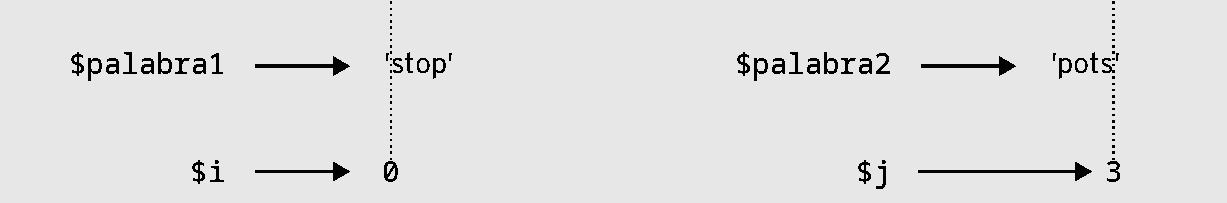
\includegraphics[scale=0.5]{figs/state6.pdf}}
\caption{Diagrama de estado.}
\label{fig.state4}
\end{figure}

Tomamos ciertas libertades para acomodar las variables en
el cuadro y agregar líneas punteadas para mostrar que los valores de
{\tt \$i} y {\tt \$j} indican caracteres en {\tt \$palabra1} y
{\tt \$palabra2}.

Comienza con este diagrama, ejecuta el programa en papel, 
cambia los valores de {\tt \$i} y {\tt \$j} durante cada iteración.
Encuentra y arregla el segundo error en esta función.

Solución: \ref{sol_isreverse}.
\label{isreverse}
\index{is-reverse}


\section{Glosario}

\begin{description}

\item[Objecto] Algo que una variable puede almacenar. 
Por el momento, puedes usar ``objeto`` y ``valor`` indistintamente.
\index{object}

\item[Secuencia] Una colección ordenada de valores donde cada valor
es identificado por un índice entero.
\index{sequence}

\item[Artículo] Uno de los valores en una secuencia.
\index{item}

\item[Índice] Un valor entero que se usa para seleccionar un
artículo en una secuencia, tal como un carácter en un cadena 
de texto. En Perl, los índices comienzan desde el 0.
\index{index}

\item[Rebanada] Una parte de una cadena de texto especificada por un
rango de índices.
\index{slice}

\item[Cadena de texto vacía] Una cadena de texto sin caracteres y con longitud 0,
representada por dos comillas.
\index{empty string}

\item[Recorrer] Iterar a través de los artículos de una secuencia,
realizando una operación similar en cada uno de ellos.
\index{traversal}

\index{search}
\item[Búsqueda] Una patrón de recorrido que para cuando encuentra
lo que está buscando.
\index{search!pattern}
\index{pattern!search}

\index{counter}
\item[Contador] Una variable que se usa para contar algo, usualmente
inicializada a cero y posteriormente incrementada.

\index{regular expression}
\item[Expresiones  regulares] Un sublenguaje de computación
derivado de la teoría de lenguajes formales.

\index{pattern}
\item[Patrón] Una secuencia de caracteres con sintaxis especial
que describen de izquierda a derecha el contenido que se intenta
coincidir dentro de una cadena de texto en particular.

\index{regex}
\item[Regexes] Un sublenguaje de coincidencia de patrón de Perl~6
derivado de las expresiones regulares.

\index{backtracking}
\item[Vuelta atrás] El proceso por el cual,
dado un intento de coincidencia fallido en una cadena de texto, el motor de regex 
abandona parte del intento de coincidencia actual, vuelve atrás
en la cadena de texto, e intenta nuevamente para ver si puede
encontrar una nueva ruta a una coincidencia exitosa. 
El proceso de vuelta atrás eventualmente para tan pronto una
coincidencia exitosa ocurre, o finalmente cuando todas las 
coincidencias posibles fallan. Este proceso se conoce como
\emph{backtracking} en inglés.

\end{description}


\section{Ejercicios}


\begin{exercise}
\label{count_a}
\index{count method}
\index{method!count}
\index{index function}

Escribe una subrutina que use la función {\tt index}  en un bucle
para contar el número de caracteres ``a`` en \verb|`banana`| como 
hicimos en la Sección~\ref{counter}. Modifícala para contar
cualquier letra en cualquier palabra pasadas como argumentos 
a la subrutina.

Escribe otra subrutina para contar una letra dada en una 
palabra dada usando la función {\tt substr}.
\index{substr function}

Solución: \ref{sol_count_a}
\end{exercise}


\begin{exercise}

\label{islower}
\index{lower case!character class}
\index{character class}
La categoría de caracteres \verb|<[a..z]>| coinciden con cualquier
carácter en minúscula (solo caracteres ASCII en minúscula, no caracteres
Unicode). La siguiente subrutina:

\begin{verbatim}[fontshape=up]
sub es-minúscula (Str $char) { 
    return so $char ~~ /^<[a..z]>$/
}
\end{verbatim}

debería devolver {\tt True} si su argumento es una letra ASCII
en minúscula y de lo contrario, {\tt False}. Asegúrate de que 
funcione como se espera (y arréglala si es necesario). La 
función {\tt so} coacciona el resultado de la coincidencia de regex 
en un valor Booleano.

Las siguientes subrutinas usan la subrutina {\tt es-minúscula}
y su trabajo es chequear si una cadena de texto contiene 
letras en minúsculas, pero algunas de ellas no funcionan 
adecuadamente. Analiza cada subrutina manualmente, 
determina si funciona bien, y describe lo que actualmente
hace (puedes asumir que el parámetro es una cadena de texto).
Después, pruébalas todas con varias cadenas de texto para chequear
si tu análisis estaba en lo cierto.

\begin{verbatim}[fontshape=up]
# ADVERTENCIA: algunas de las siguientes subrutinas
#              no funcionan correctamente.

sub cualquier_minúscula1(Str $cadena){
    for $cadena.comb -> $char {
        if es-minúscula $char {
            return True;
        } else {
            return False;
        }
    }
}

sub cualquier_minúscula2(Str $cadena){
    for $cadena.comb -> $char {
        if es-minúscula "char" {
            return True;
        } else {
            return False;
        }
    }
}

sub cualquier_minúscula3(Str $cadena){
    my $flag;
    for $cadena.comb -> $char {
        $flag =  es-minúscula $char;
    }
    return $flag;
}

sub cualquier_minúscula4(Str $cadena){
    my $bandera = False;
    for $cadena.comb -> $char {
        $bandera = $bandera or es-minúscula $char;
    }
    return $bandera;
}

sub cualquier_minúscula5(Str $cadena){
    my $flag = False;
    for $cadena.comb -> $char {
        if es-minúscula $char {
            $flag = True;
        }
    }
    return $flag;
}

sub cualquier_minúscula6(Str $cadena){
    for $cadena.comb -> $char {
        if es-minúscula $char {
            return 'True';
        }
    }
    return 'False';
}

sub cualquier_minúscula7(Str $cadena){
    for $cadena.comb -> $char {
        return True if es-minúscula $char;
    }
    return False;
}

sub cualquier_minúscula8(Str $cadena){
    for $cadena.comb -> $char {
        return False unless es-minúscula $char;
    }
    return True;
}

sub cualquier_minúscula9(Str $cadena){
    for $cadena.comb -> $char {
        if not es-minúscula $char {
            return False;
        }
    return True;
    }
}
\end{verbatim}

Solución: \ref{sol_islower}.

\end{exercise}


\begin{exercise}
\index{letter rotation}
\index{rotation, letter}
\index{Caesar cipher}

\label{rotate}
Un cifrado César es una forma débil de cifrado que involucra
la ``rotación`` de cada letra por un número fijo de posiciones.
La rotación de una letra se refiere a su desplazamiento a través
del alfabeto, y puede envolverse alrededor si es necesario, 
así que ``A`` rotada por 3 corresponde a ``D`` y ``Z`` rotada por
1 corresponde a ``A``.

Para rotar una palabra, rota cada letra por el mismo número de posiciones.
For ejemplo, ``educar`` rotada por 7 es ``lkbjhy`` y ``carta`` rotada por 
-10  es ``sqhjq``. (Para el cifrado, usamos solo caracteres del alfabeto
básico latino ISO.) En la película
{\em 2001: A Space Odyssey}, la computadora de la nave se llama 
HAL, que es una rotación de IBM por -1.

Escribe una función llamada \verb|rotar-palabra| que toma una cadena de texto
y un número entero como parámetros, y devuelve una nueva cadena que 
contiene las letras de la cadena original rotadas por el monto dado.


Podrías querer utilizar las funciones integradas {\tt ord}, 
la cual convierte un carácter a su código numérico (Unicode code point),
y {\tt char}, la cual convierte tales código numérico devuelta los
caracteres:
\index{ord function}
\index{chr function}
\index{function!ord}
\index{function!chr}

\begin{verbatim}[fontshape=up]
> say 'c'.ord;
99
> say chr 99
c
\end{verbatim}
%

Las letras del alfabeto están codificadas en orden 
alfabético, así que por ejemplo:
\index{alphabetic order}

\begin{verbatim}[fontshape=up]
> ord('c') - ord('a')
2
\end{verbatim}

dado que \verb|'c'| es la segunda letra después de \verb|'a'|
en el alfabeto. Pero ten pendiente: los códigos numéricos para
las letras mayúsculas son diferentes.
\index{upper case}
\index{case!upper}

\index{rot13}
Bromas en la Internet que tienen el potencial de ser ofensivas
son algunas veces codificadas en ROT13, el cual es un cifrado 
César con rotación 13. Dado que 13 es la mitad del número de letras
en nuestro alfabeto, la aplicación de una rotación por 13 devuelve la
palabra original, así que el mismo procedimiento puede usarse
para cifrar y descifrar en rotación 13. Si no te ofendes fácilmente,
encuentra y descifra algunas de estas bromas. (ROT13 se usa también 
para otros propósitos, tales como ocultar débilmente la solución de
un acertijo.)

Solución: \ref{sol_rotate}.

\end{exercise}

